\documentclass[12pt, letterpaper]{report}
\usepackage[hidelinks]{hyperref}
\usepackage{graphicx}
\graphicspath{ {./} }
\usepackage[rightcaption]{sidecap}
\hypersetup{
	pdftitle={},    % title
	pdfauthor={},     % author
	pdfsubject={},   % subject of the document
	pdfcreator={},   % creator of the document
	pdfproducer={},  % producer of the document
	pdfkeywords={}, % list of keywords
	pdfcreationdate={},
	pdfmoddate={}
%     pdfnewwindow=true,      % links in new window
}

\usepackage{listings}

\lstset{%
  language=bash,
  basicstyle=\fontfamily{pcr}\selectfont,
  commentstyle=\bfseries,
  escapeinside={(*@}{@*)}
}
\usepackage{titlesec}
\title{AP Compsci: Personal Project}
\author{Written by Alex Colley}

\begin{document}
\maketitle
\tableofcontents
\newpage
% \begin{abstract}
\addcontentsline{toc}{chapter}{Abstract}
\chapter*{Abstract}
	This is a command line Java encoding tool written for my AP Compsci class that
uses base64 encoding to encode inputted data. It implements a relatively advanced CLI,
and will assist with putting files with non-readable characters into readable characters. 
\addcontentsline{toc}{chapter}{Introduction}
\chapter*{Introduction}
	Base64 is a commonly used algorithm designed to convert binary files into files that
can actually be viewed. The objective of this program is to take text that is inputted by
the user, and then to output that is the input converted into base64.


\chapter{CLI} \label{chapter:1}
\section{Commands} \label{sec:1:1}
	The Command class is a class meant to simulate a command that can be ran by the 
	CLI. It is implemented in CLI.java
\subsection{Members} \label{sec:1:1:1}
	The Command class has 3 members:
\begin{lstlisting}[breaklines=true, language=Java, label=code:1:1:1:1]
	private Function<Map<String, String[]>, Integer> function;
	private int argsRequired;
	private String help;
\end{lstlisting}
Where function is the function that the command calls when it is ran, argsRequired is the
number of args required by the command, and help is the description of the command and how
to use it.
\subsection{Constructor}
The Command class is initialized like so:
\begin{lstlisting}[breaklines=true, language=Java, label=code:1:1:2:1]
	public Command(Function<Map<String, String[]>, Integer> function, int argsRequired, String help)


	{


		this.help = help;
		this.function = function;
		this.argsRequired = argsRequired;


	}  //  public Command(Function<Map<String, String[]>, Integer> function, int argsRequired)

\end{lstlisting}
or 
\begin{lstlisting}[breaklines=true, language=Java, label=code:1:1:2:2]
	public Command(Function<Map<String, String[]>, Integer> function, int argsRequired)


	{


		this.help = "";
		this.function = function;
		this.argsRequired = argsRequired;


	}  //  public Command(Function<Map<String, String[]>, Integer> function, int argsRequired)
\end{lstlisting}
This sets each member for later use. 
\subsection{The runCommand function}
The function in this.function is only called when the runCommand method is called:
\begin{lstlisting}[breaklines=true, language=Java, label=code:1:1:3:1]
	public Integer runCommand(Map<String, String[]> args)


	{


		if ( args.size() < this.argsRequired )
			return -1;
		return this.function.apply(args);


	}  //  public Integer runCommand(String arg)
\end{lstlisting}
Where args is a hashmap of options to be sent to the command.
\subsection{The getters}
The getArgsRequired method is a getter method which returns the argsRequired member:
\begin{lstlisting}[breaklines=true, language=Java, label=code:1:1:4:1]
	public int getArgsRequired()


	{

	
		return this.argsRequired;


	}
\end{lstlisting}
And the getHelp method is a getter method which returns the help member:
\begin{lstlisting}[breaklines=true, language=Java, label=code:1:1:4:2]
	public String getHelp()


	{


		return this.help;


	}  //  public String getHelp()
\end{lstlisting}
This class will be used the following class to actually run commands specified by the user.
\section{The CLI Class}
\subsection{members}
	The Command class has 3 members:
\begin{lstlisting}[breaklines=true, language=Java, label=code:1:2:1:1]
	private Map<String, Command> commands;
	private String[] args;
	private String currentCommand;
\end{lstlisting}
Where commands is a hashmap of a String, which is the name of a Command, mapped to a Command object.
The currentCommand member refers to the command being ran by the user in the terminal to invoke the program, e.g. java package.class. 
This is not referring to an instantiation of the Command class, and is meant to be used for the usage method.
\subsection{Constructor}
The CLI class is initialized like so:
\begin{lstlisting}[breaklines=true, language=Java, label=code:1:2:2:1]
	public CLI(String[] args, Map<String, Command> commands, String currentCommand)


	{


		this.commands = commands;
		this.args = args;
		this.currentCommand = currentCommand;


	}  //  public CLI(String[] args)
\end{lstlisting}
\subsection{The getInput method}
The getInput method is a method that accepts user input typically from a pipe($|$). It is meant to be
used to input entire files for encoding. It is a static method, and does not require an associated CLI
object. It is implemented like so:
\begin{lstlisting}[breaklines=true, language=Java, label=code:1:2:3:1]
	public static String getInput()


	{


		BufferedReader reader = new BufferedReader(new InputStreamReader(System.in));
		Scanner scanner = new Scanner(System.in);
		StringBuilder stringBuilder = new StringBuilder();


		while ( scanner.hasNextLine() )


		{
			

			stringBuilder.append(scanner.nextLine());
			stringBuilder.append(System.lineSeparator());
			

		}  //  while ( scanner.hasNextLine() )


		stringBuilder.deleteCharAt((stringBuilder.length() - 1));
		scanner.close();
		String input = stringBuilder.toString();
		return input;


	}  //  public static String getInput()
\end{lstlisting}
\subsection{The usage method}
The usage method, which is referenced above, prints out how exactly the program is to be invoked:
\begin{lstlisting}[breaklines=true, language=Java, label=code:1:2:4:1]
	public void usage()


	{


		System.out.printf("Usage: %s [command] [options]\n", this.currentCommand);
		System.out.printf("Commands:\n");
		for (Map.Entry<String, Command> entry : this.commands.entrySet())
			System.out.printf("\t%s: %s\n", entry.getKey(), entry.getValue().getHelp());


	}  //  public void usage()
\end{lstlisting}
This is in case the user invokes the program incorrectly.
\subsection{The run method}
The run method is instantiated like so:
\begin{lstlisting}[breaklines=true, language=Java, label=code:1:2:5:1]
	public void run()


	{


		if ( this.args.length == 0)


		{


			this.usage();
			return;


		}  //  if ( this.args.length == 0 )


		String commandName = this.getCommandName();


		if ( !this.commands.containsKey(commandName) )


		{


			System.out.printf("Error: no such command %s\n", commandName);
			this.usage();
			return;


		}  //  if ( this.commands.containsKey(commandName) )


		Command command = this.commands.get(commandName);
		Map<String, String[]> arguments = new HashMap<>();


		if ( this.args.length < command.getArgsRequired() )


		{


			System.out.printf("My commands don't have arguments for this project.");
			return;


		}  //  if ( this.args.length < command.getArgsRequired() )


		command.runCommand(arguments);


	}  //  public void run()
\end{lstlisting}
The code checks that the program actually got a command to run, and if it didn't,
it calls the usage method and returns. If it did get a command to run, it ensures
that the program has the command specified by checking to see if the hashmap which
contains the list of commands has a key with the same name as the command provided.
If it doesn't, it prints out an error, and calls usage again. If it does, it ensures
that the minimum amount of command line arguments\footnote{The amount of command line arguments required for all Commands are 0, as none of the Command functions require information outside of the stdin input.} were supplied, and calls the runCommand
method of the Command object pointed to on the hashmap by the key.
\subsection{The getters}
This class has one getter, entitled get command name, which returns the 0th member of the args member:
\begin{lstlisting}[breaklines=true, language=Java, label=code:1:2:6:1]
	public String getCommandName()


	{


		return this.args[0];


	}  //  public String getCommandName()
\end{lstlisting}
\chapter{The base64 encoding} \label{chapter:2}
\section{The B64Encoding class}
The base64 encoding is implemented in its own B64Encoding.java, which contains one class with the name
B64Encoding. The B64Encoding.java imports java.util.Base64 and establishes the current package.
\begin{lstlisting}[breaklines=true, language=Java, label=code:2:1:0:1]
package src;
import java.util.Base64;
\end{lstlisting}
for use in the B64Encoding class.
The B64Encoding class is a class with methods intended to perform base64 encoding and decoding operations.
It has one member:
\begin{lstlisting}[breaklines=true, language=Java, label=code:2:1:0:2]
	private String message;
\end{lstlisting}
which is the data to encode. The member is assigned a vaue in one of 2 constructors:
\begin{lstlisting}[breaklines=true, language=Java, label=code:2:1:0:3]
	public B64Encoding()


	{


		this.message = "";


	}  //  public B64Encoding() 
\end{lstlisting}
or
\begin{lstlisting}[breaklines=true, language=Java, label=code:2:1:0:4]
	public B64Encoding(String message)


	{


		this.message = message;


	}  //  public B64Encoding(String message)
\end{lstlisting}
\subsection{The update and clear methods}
The private message member can be modified with 2 different methods.
The update method concatenates a new string on to the message member:
\begin{lstlisting}[breaklines=true, language=Java, label=code:2:1:1:1]
	public void update(String addition)


	{


		this.message+=addition;


	}  //  public void update(String addition)
\end{lstlisting}
The clear method sets the message member to an empty string:
\begin{lstlisting}[breaklines=true, language=Java, label=code:2:1:1:2]
	public void clear()


	{


		this.message = "";


	}  //  public void clear()
\end{lstlisting}
\subsection{The encode method}
The encode method returns the base64 encoded message member:
\begin{lstlisting}[breaklines=true, language=Java, label=code:2:1:2:1]
	public String encode()


	{


		return Base64.getEncoder().encodeToString(this.message.getBytes());


	}  //  public String encode()
\end{lstlisting}
\subsection{The decode method} \label{sec:2:1:3}
The decode method takes no arguments, and returns a string that is the
message member decode from base64:
\begin{lstlisting}[breaklines=true, language=Java, label=code:2:1:3:1]
	public String decode()


	{


		return new String(Base64.getDecoder().decode(this.message.getBytes()));


	}  //  public String encode()
\end{lstlisting}
\section{The Commands}
The program has 3 commands that are associated
with a string, and can be invoked via a command
line argument. 
\subsection{The b64encode function}
The b64encode function takes in a string from stdin, and outputs the 
string encoded with base64. It is implemented like so:
\begin{lstlisting}[breaklines=true, language=Java, label=code:2:2:1:1]
	public static Integer b64encode(Map<String, String[]> kwargs)


	{


		String message = CLI.getInput();
		B64Encoding b64 = new B64Encoding(message);
		System.out.printf("%s", b64.encode());
		return 1;


	}  //  public static Integer b64encode(Map<String, String[]> kwargs)
\end{lstlisting}
\chapter{The Main File.}
The main file is mainacv01.java. It has one class
with 3 methods.
\section{The main method}
The main method is a simple method that takes the arguments provided by the user,
lists the functionality of the program, and calls the run function implemented
in \ref{code:1:2:5:1}:
\begin{lstlisting}[breaklines=true, language=Java, label=code:3:1:0:1]
	public static void main(String[] args)


	{


		// kwargs.put("testCommand", new Command("testCommand", mainacv01::testCommand, 0));
		// System.out.printf("%s\n", CLI.getInput());
		Map<String, Command> commands = new HashMap<>();
		commands.put("encode", new Command(mainacv01::b64encode, 0, "Encode a string with base64."));
		commands.put("decode", new Command(mainacv01::b64decode, 0, "Decode base64 encoding."));
		CLI cli = new CLI(args, commands, "java final2WeeksProject.mainacv01");
		cli.run();


	}  //  public static void main(String[] args)
\end{lstlisting}
\section{The b64encode method}
The b64encode method uses the encode method implemented in \ref{code:2:1:2:1} and 
the getInput method implemented in \ref{code:1:2:3:1} to encode data. It is implemented
like so:
\begin{lstlisting}[breaklines=true, language=Java, label=code:3:2:0:1]
	public static Integer b64encode(Map<String, String[]> kwargs)


	{


		String message = CLI.getInput();
		// System.out.printf("%s", message);
		B64Encoding b64 = new B64Encoding(message);
		System.out.printf("%s\n", b64.encode());
		return 1;


	}  //  public static Integer b64encode(Map<String, String[]> kwargs)
\end{lstlisting}

\section{The b64decode method}
The encode method uses the decode method implemented in \ref{code:2:1:3:1} and 
the getInput method implemented in \ref{code:1:2:3:1} to decode data. It is implemented
like so:
\begin{lstlisting}[breaklines=true, language=Java, label=code:3:3:0:1]
	public static Integer b64decode(Map<String, String[]> kwargs)


	{


		String message = CLI.getInput();
		// System.out.printf("%s", message);
		

		try


		{
			

			B64Encoding b64 = new B64Encoding(message);
			System.out.printf("%s\n", b64.decode());
			

		}  //  try 


		catch(java.lang.IllegalArgumentException e)


		{


			System.err.printf("The text provided was not encoded with base64.");


		}  //  catch(java.lang.IllegalArgumentException e)


		return 1;


	}  //  public static Integer b64decode(Map<String, String[]> kwargs)
\end{lstlisting}


\chapter{Running the program}
\section{Requirements}
	As this project was coded in Java, the user must have a Java runtime installed
on their machine. 
\section{Commands and outputs}
\subsection{Running the Program With No Arguments}
When ran with no arguments, the program gives the following output:


% \begin{SCfigure}[0.5][h]
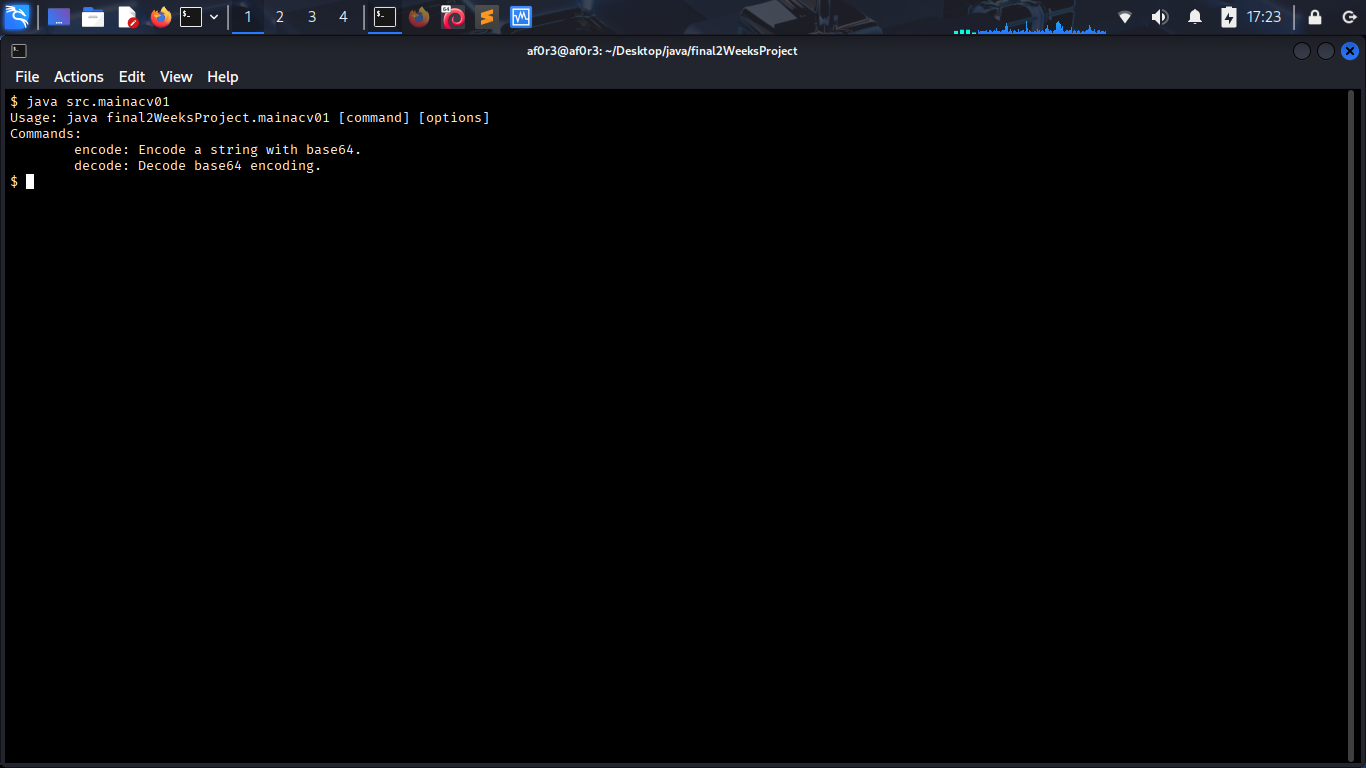
\includegraphics[width=1\textwidth]{noarguments}
% \end{SCfigure}

	This is the output of the usage method implemented
in \ref{code:1:2:4:1}.
\subsection{Using the program to encode data}
The program can be used to encode data to base64 like the example
below:

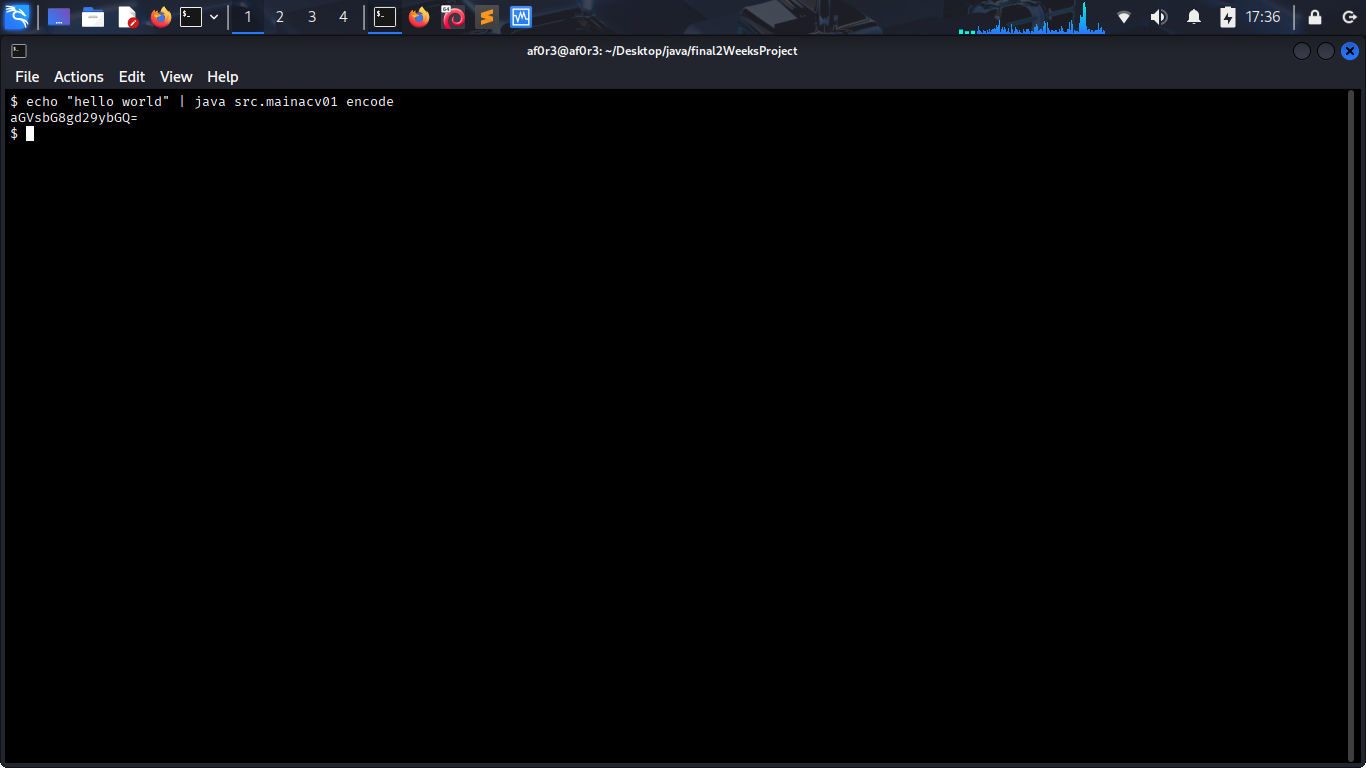
\includegraphics[width=1\textwidth]{encode}

If the data is not given to the program through a pipe to stdin, the
program will simply wait for input forever.

\subsection{Using the program to decode data}
The program can be used to decode data from base64 like the example
below:

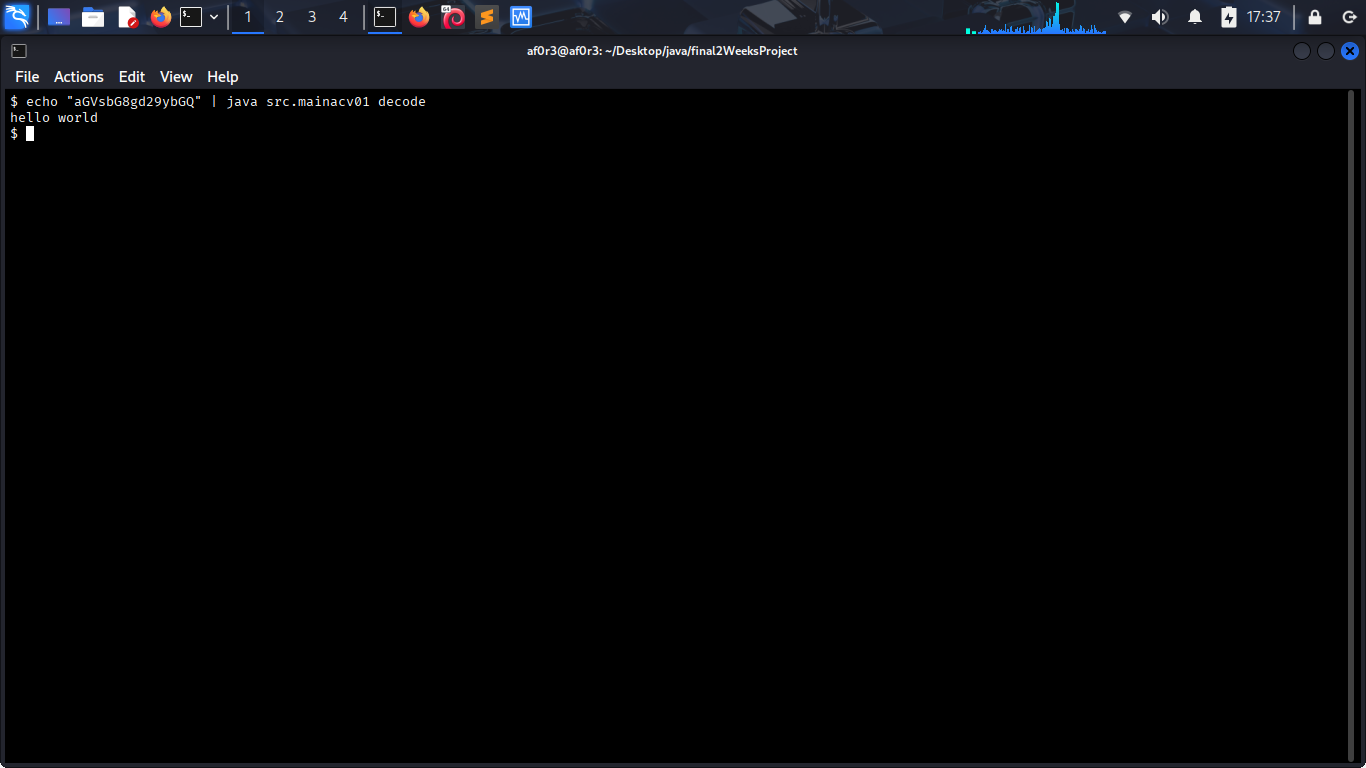
\includegraphics[width=1\textwidth]{decode}

Once again, the data must be given to the program through a pipe to stdin.

\addcontentsline{toc}{chapter}{Conclusions}
\chapter*{Conclusions}
	This was my first command line program in java that actually takes input from
the user with command line arguments, and the first ever coding project that I
have taken upon myself that involved documentation. This has taught me a lot about
writing, organizing, and documenting code.

\end{document}

